\documentclass[../../../interview-questions.tex]{subfiles}

\begin{document}

\subsection{MySQL组合索引(Multiple-Column Indexes)为什么最左匹配}

构建一颗 B+ 树只能根据一个值来构建,因此数据库依据联合索引最左的字段来构建 B+ 树。B+树的数据项是复合的数据结构,如图\ref{fig:multicolumnindex}所示,仔细观察索引结构,可以看到索引key在排序上,首先按a排序,a相等的节点中,再按b排序。因此,如果查询条件是a或a和b联查时,是可以应用到索引的。如果查询条件是单独使用b,因为无法确定a的值,因此无法使用索引。

\begin{figure}[htbp]
    \centering
    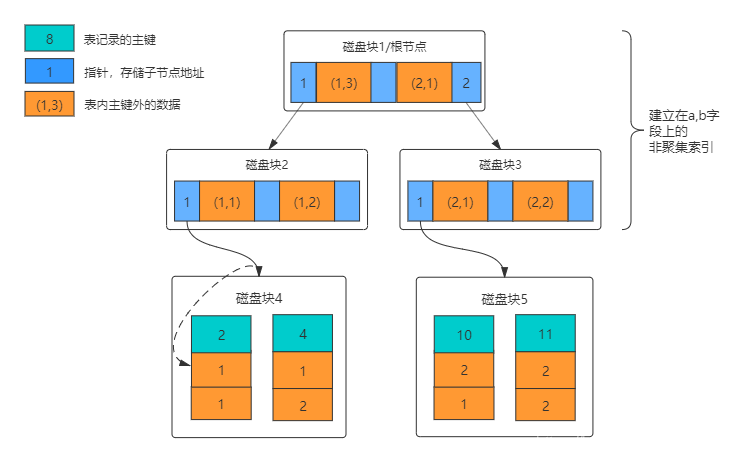
\includegraphics[scale=0.35]{multicolumnindex.png}
    \caption{组合索引存储结构}
    \label{fig:multicolumnindex}
\end{figure}

比如(name,age,sex)的时候,B+树是按照从左到右的顺序来建立搜索树的,比如当(张三,20,F)这样的数据来检索的时候,B+树会优先比较name来确定下一步的搜索方向,如果name相同再依次比较age和sex,最后得到检索的数据;但当(20,F)这样的没有name的数据来的时候,B+树就不知道第一步该查哪个节点,因为建立搜索树的时候name就是第一个比较因子,必须要先根据name来搜索才能知道下一步去哪里查询。
比如当(张三,F)这样的数据来检索时,B+树可以用name来指定搜索方向,但下一个字段age的缺失,所以只能把名字等于张三的数据都找到,然后再匹配性别是F的数据了, 这个是非常重要的性质,即索引的最左匹配特性。
联合索引(col1, col2,col3)也是一棵B+Tree,其非叶子节点存储的是第一个关键字的索引,而叶节点存储的则是三个关键字col1、col2、col3三个关键字的数据,且按照col1、col2、col3的顺序进行排序。联合索引(年龄, 姓氏,名字),叶节点上data域存储的是三个关键字的数据。且是按照年龄、姓氏、名字的顺序排列。因为联合索引(Multiple-Column Indexes\footnote{参见:\url{https://dev.mysql.com/doc/refman/5.7/en/multiple-column-indexes.html}})中是先根据年龄进行排序的。如果年龄没有先确定,直接对姓氏和名字进行查询的话,就相当于乱序查询一样,因此索引无法生效。因此查询是全表查询。而之所以会有最左原则,是因为联合索引的B+Tree是按照第一个关键字进行索引排列的。





\end{document}